% Section content template for individual Educative lessons
% This file contains the actual content for a specific section
% Generated from Educative API section content

% Section: Dropbox System Design
% Section ID: 6405132675579904
% Section Slug: dropbox-system-design
% Generated: 2025-12-08T15:51:08.583083

Dropbox is a cloud-based file storage and synchronization service that allows users to store, share, and collaborate on files across multiple devices.
\\
When a file is added or modified in a Dropbox folder, the system ensures that all connected devices and collaborators have access to the most up-to-date version. This requires efficient storage, synchronization, and metadata management, as well as secure authentication and access control.
\\
Dropbox is one of several cloud storage and collaboration tools available today, alongside:

\begin{itemize}
\item
\protect\phantomsection\label{sY7LNhE-RgIpUUGpjkEq8}
Google Drive
\item
\protect\phantomsection\label{rVCnJCWxNSkdE01VpK6DI}
Microsoft OneDrive
\item
\protect\phantomsection\label{gNeRvOhErN8idpQ2taBTE}
Box
\item
\protect\phantomsection\label{FdYkCVsAfZUDN3SnO-AV5}
Jupyter
\end{itemize}
\\
As of November 2023, Google Drive held the largest market share in cloud storage, with Dropbox in second place. Dropbox 's continued adoption demonstrates its focus on reliable synchronization, simplicity, and scalability, particularly for collaborative workflows.

\textbf{Market Share of File Sharing Systems}

\textit{\small [Chart data presented in table format]}

\begin{table}[htbp]
\centering
\small
\adjustbox{max width=\textwidth}{
\begin{tabular}{|p{0.475\textwidth}|p{0.475\textwidth}|}
\hline
\textbf{Label} & \textbf{Percentage Market Share} \\
\hline
\hline
Google Drive & 31.19 \\
\hline
Dropbox & 18.61 \\
\hline
OneDrive & 14.84 \\
\hline
Box & 12.96 \\
\hline
Jupyter & 8.45 \\
\hline
Other & 13.95 \\
\hline
\end{tabular}
}
\caption{The market share of top 5 file synchronization and sharing services}
\end{table}

\subsection{Requirements}\label{rwUPYXIJJuhAtnvHlnm1j}
\\
Defining requirements is a crucial first step in designing a system like Dropbox. Requirements are typically categorized as either functional or nonfunctional, providing a clear scope for the design process.

% \vspace{-1.0\baselineskip}
\noindent
\begin{minipage}[t]{0.48\textwidth}\vspace{0pt}
\textbf{Functional Requirements}
\begin{itemize}
    \item Upload files
    \item Download files
    \item Share files/directories
    \item Create and delete directories
    \item Synchronization upon file changes
    \item Version control for files
    \item User authentication and access control
\end{itemize}
\end{minipage}
\hfill
\begin{minipage}[t]{0.48\textwidth}\vspace{0pt}
\textbf{Nonfunctional Requirements}
\begin{itemize}
    \item Durability and reliability
    \item Availability
    \item Scalability
    \item Security
    \item Low-latency file retrieval
\end{itemize}
\end{minipage}
\\
\\
Clarifying requirements is also essential in System Design interviews, as it demonstrates a structured approach to understanding the problem scope. For example, distinguishing between functional and nonfunctional requirements provides guidance for both the backend architecture and the client-side design.
\\
After requirements are established, it is necessary to estimate the system resources required to support expected user activity. This includes determining storage, bandwidth, and server capacity.

\subsection{Resource estimation for Dropbox architecture}\label{a6EOvVej4C14Y3smSMzcu}
\\
Resource estimation involves calculating storage, bandwidth, and server requirements based on projected user activity. For this analysis, assume Dropbox has 50 million paying users.
\begin{quote}
\textbf{Note:} According to Backlinko(https://backlinko.com/dropbox-users), Dropbox had approximately 18.22 million paying users as of Q2 2024. Designing for 50 million users allows planning for future growth.
\end{quote}
\subsubsection{Storage estimation}\label{-VJ8fUYeuguHQiicz1s8Q}
\\
If each user is allocated 2 TB of storage, the total storage requirement is calculated as:

\begin{align*}
\text{Total storage} &= \text{Number of users} \times 2 \text{ TB} \\
&= 50 \times 10^6 \times 2 \text{ TB} \\
&= 100 \times 10^6 \text{ TB} \\
&= 100 \text{ PB}
\end{align*}


Thus, the system would require approximately 100,000 petabytes of storage to accommodate 50 million users.

\subsubsection{Bandwidth estimation}\label{p26uukah1nxvr-GkdXZ0p}
\\
Assuming that each user consumes 1 GB of bandwidth per day, the total bandwidth requirement can be estimated as:

\begin{align*}
\text{Total bandwidth} 
&= 50 \times 10^6 \times 1 \text{ GB} \\
&= 50 \text{ EB/day} \\
&= \frac{50 \text{ EB}}{24 \times 60 \times 60 \text{ s}} \\
&\approx 579 \text{ GB/s} \\
&= \frac{579 \text{ GB/s}}{8} \\
&\approx 72.5 \text{ Gbps}
\end{align*}


This calculation provides a baseline for network infrastructure to support daily user operations.

\subsubsection{Server estimation}\label{GLgXog-otuOLzfgmHhhoe}
\\
To estimate server requirements, first calculate the queries per second (QPS). Assuming each active user sends 5 requests per minute:

\[
\text{QPS} = \frac{50 \text{ M} \times 5 \text{ requests}}{60} = 4.2 \text{ M}
\]

\begin{quote}
\textbf{Note:} According to the \href{https://www.educative.io/blog/back-of-envelope-estimation-system-design-interview}{back-of-the-envelope estimations}, a 64-core server executes approximately 64000 requests per second.
\end{quote}
\\
Considering that a 64-core server can handle approximately 64,000 requests per second, the required number of servers is:

\[
\text{Number of servers} = \frac{4.2 \text{ M}}{64000} \approx 66 \text{ servers}
\]

So, to summarize, for 50 M users, the following is the estimation for different resources:

\begin{itemize}
\item
\protect\phantomsection\label{9PQcS3uvJa1YRm6I2DBuj}
Estimated storage = \protect\phantomsection\label{katex_inline_lrNacJYwOXKAWHhBRezRw}{{{\(100 \text{ EB}\)}}}
\item
\protect\phantomsection\label{m_QJLaulc7GKRK752PPJz}
Estimated bandwidth = \protect\phantomsection\label{katex_inline_qmcE7k5WeZeY_hxHb48Qa}{{{\(72.5 \textrm{ Gbps}\)}}}
\item
\protect\phantomsection\label{5yE-I021HmryrCXau91KA}
QPS = \protect\phantomsection\label{katex_inline_C9gcRit0kr0SLSB2AKNYl}{{{\(4.2\text{ M}\)}}}
\item
\protect\phantomsection\label{jWv_sTuQa0PWUfqgs2VRf}
The number of servers = \protect\phantomsection\label{katex_inline_k4vljrxHmM9CfcSKA9saJ}{{{\(66 \text{ servers}\)}}}
\end{itemize}
\\
You can estimate these resources for different numbers of users in this calculator:

These estimations provide a foundation for designing storage, networking, and server infrastructure to support anticipated user demand.

\subsection{High-level design of Dropbox}\label{rCGmQBfajIvlUxvqPlJhK}
\\
The high-level architecture of Dropbox consists of multiple interacting components and services that manage file storage, metadata, synchronization, and access control. Key components include:

\begin{itemize}
\item
\protect\phantomsection\label{K2jCcZ74KHbOIW-DmyGiQ}
\textbf{Metadata service:} Maintains information about files, directories, and user activity.
\item
\protect\phantomsection\label{cParbi9n1rJnHGwqLx4gI}
\textbf{Chunk service (chunker):} Responsible for splitting files into chunks and handling their storage and retrieval from cloud storage.
\item
\protect\phantomsection\label{D-WAdhG6lbuzjirvVy6iH}
\textbf{Metadata database:} Stores metadata, including file paths, versions, ownership, and access permissions.
\item
\protect\phantomsection\label{otCtBDNBsy8iUq6qzf4U8}
\textbf{Cloud storage:} Provides scalable, distributed storage for encrypted file chunks.
\item
\protect\phantomsection\label{C7swO4Dm0lWVLSZ0pZsvX}
\textbf{Synchronization service:} Coordinates file updates across multiple devices, ensuring consistency and notifying collaborators of changes.
\end{itemize}
\\
The overall system ensures that when a user uploads or modifies a file, the metadata service, chunk service, and synchronization service collaborate to update cloud storage and propagate changes to all devices associated with the user\textquotesingle s account.
\\
Replication and redundancy mechanisms ensure high availability and durability.

\begin{figure}[htbp]
 \centering
 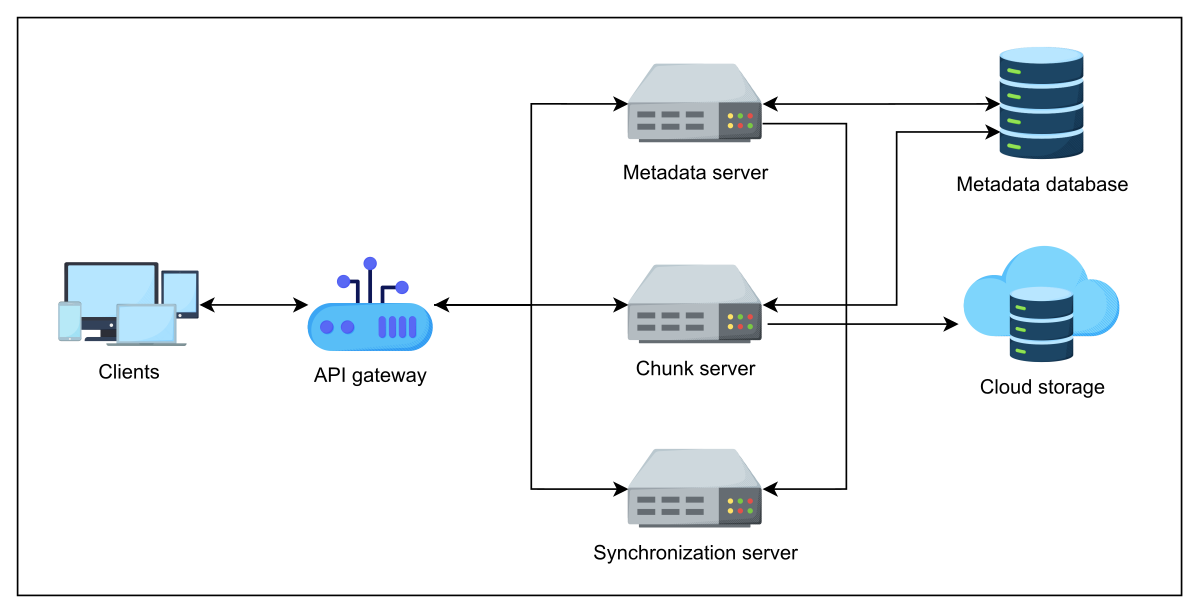
\includegraphics[width=0.5\textwidth]{Images/chapter_45/section_6405132675579904/5250611425443840.png}
 \caption{A high-level design of Dropbox system}
\end{figure}

This high-level view provides a foundation for the detailed design, where each functional requirement is mapped to specific components and interactions.

\subsection{Detailed design of Dropbox}\label{CGcJBblickRHQc-5pZsB2}
\\
Let's dive into Dropbox's detailed System Design by starting with each functional requirement. We 'll discuss how to achieve each functionality step by step and the architectural changes necessary to support it.

\subsubsection{File upload and download}\label{9Zv-ybjv8PQK7ZZW1ptQk}
\\
The upload process begins when a user places a file in the client application's Dropbox folder. The file is divided into smaller chunks, typically 4 MB each. Each chunk is hashed using SHA-256, producing a unique identifier, and encrypted with AES-256 before storage. The encrypted chunks are distributed across multiple servers to ensure high availability.

\begin{figure}[htbp]
 \centering
 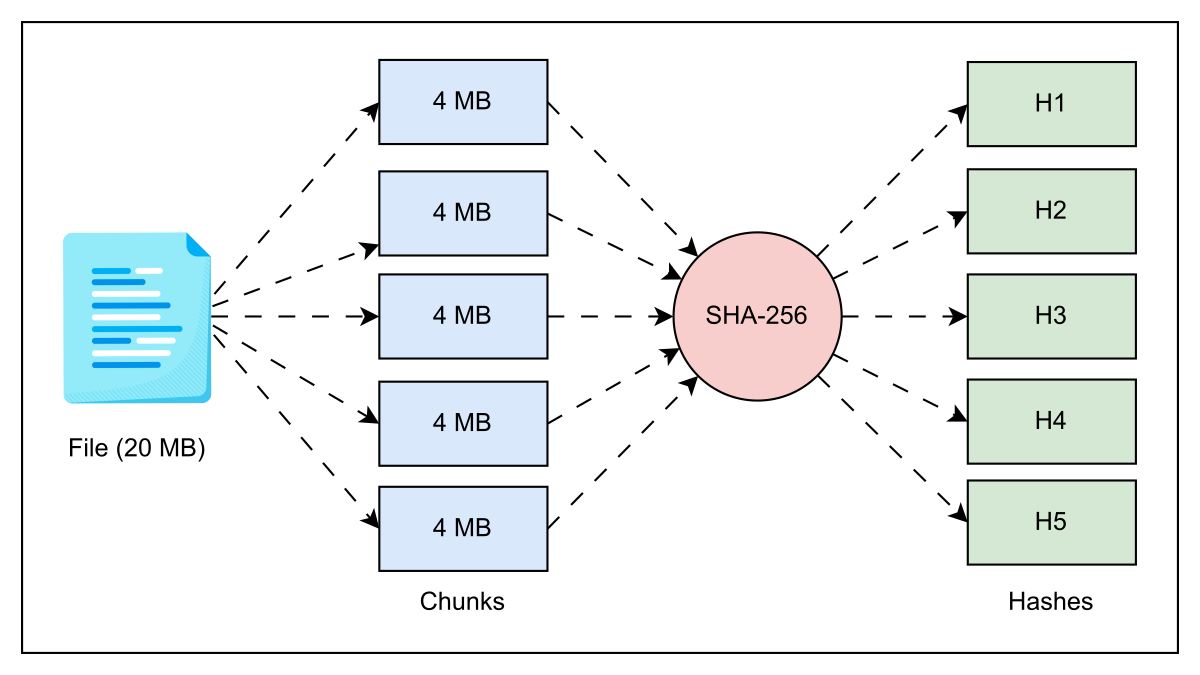
\includegraphics[width=0.5\textwidth]{Images/chapter_45/section_6405132675579904/5700418937946112.png}
 \caption{The process of dividing a file into chunks and then computing hashes}
\end{figure}

The client application coordinates with the chunk server, synchronization service, and cloud storage to manage uploads, downloads, and synchronization. During downloads, encrypted chunks are retrieved, decrypted locally, and reassembled. Caching and compression techniques are used to enhance transfer speeds and minimize server load.
\\
The following pseudo-code shows the chunking process and computing their SHA-256:

\textbf{Pseudo code for creating chunks and computing their hashes using SHA-256}

\begin{lstlisting}[language=SQL]
IMPORT SHA256 from cryptography library

FUNCTION create_file_chunks_with_hash(file_path, chunk_size):
    INITIALIZE empty list called 'chunks'
    INITIALIZE empty list called 'hashes'
    
    OPEN file at file_path in binary read mode
    SET file_position to 0
    
    WHILE file_position is less than file size:
        READ next chunk of chunk_size bytes from file
        APPEND the chunk to 'chunks'
        
        COMPUTE hash of the chunk using SHA256
        APPEND the hash to 'hashes'
        
        INCREMENT file_position by chunk_size
\end{lstlisting}

\begin{quote}
\textbf{Explanation of the above pseudo-code:}

\begin{itemize}
\item
\protect\phantomsection\label{BAaoBuXCSsZ3MfwrLSQXN}
\textbf{Line 1:} Load the SHA256 library.
\item
\protect\phantomsection\label{hC2IL36w9pmnwTHtZan1t}
\textbf{Lines 3--20:} Define a function that takes two parameters as input: the file path and the chunk size. This function returns a list of chunks and their hashes.
\item
\protect\phantomsection\label{2Cv2BSsoccGaYCV5lzb3q}
\textbf{Lines 7--17:} Open a file located at file\_path for reading in binary mode, and the file\_position is set to 0 to ensure that the entire file is processed chunk by chunk. Next, the file is read chunk-wise using a loop, and each chunk is appended to a list. Also, the SHA-256 hash is computed for each chunk and appended to the hash list.
\item
\protect\phantomsection\label{w9kC0cRikaTYr6S_6Yc6u}
\textbf{Lines 19--20:} Once the file is read, it is closed, and the lists of chunks and hashes are returned.
\end{itemize}
\end{quote}
\\
The chunk server validates each chunk by comparing its hash to existing entries. If a chunk already exists, it is not stored again. During downloads, chunks are retrieved and reassembled before delivery to the client.

\subsubsection{File sharing}\label{5F435YICG2iEGXTSMBLpl}
\\
When a user shares a file or folder, the sharing service generates a unique link or sends invitations to designated collaborators. The service enforces permissions such as \emph{read-only} or \emph{can edit} to control the level of access granted to each participant. All associated metadata, including ownership details, access control lists (ACLs), creation and modification timestamps, and permission settings, is stored and managed within the metadata service.

\subsubsection{User authentication and access control}\label{A8fDbX7ZK83nq_dhzizoe}
\\
In a system like Dropbox, user authentication and access control are crucial to ensuring that only authorized users can access files and perform specific actions. These tasks are managed through several components, including the authentication server, authorization server, and access control mechanisms.

\begin{itemize}
\item
\protect\phantomsection\label{zZ2AsdyF-nYQ99qGukXde}
\textbf{Authentication:} Supports username/password, OAuth 2.0, and multi-factor authentication (MFA). MFA adds an additional verification layer, such as a one-time password.
\item
\protect\phantomsection\label{5AZGa6lX8zd4ayo-Kor6q}
\textbf{Authorization:} Manages access based on role-based access control (RBAC), assigning permissions according to user roles (e.g., owner, editor, viewer).
\end{itemize}

\begin{figure}[htbp]
 \centering
 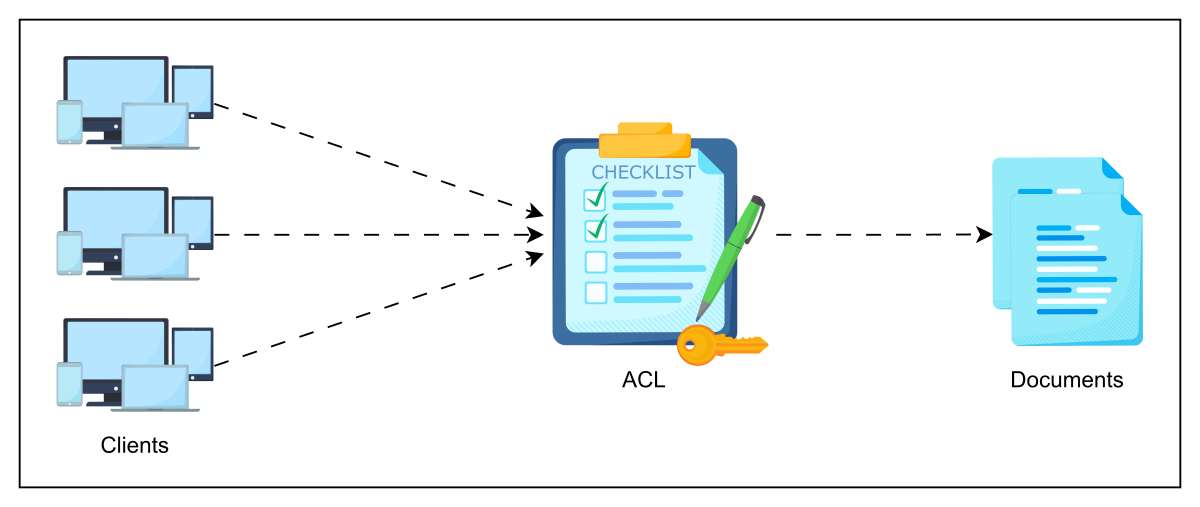
\includegraphics[width=0.5\textwidth]{Images/chapter_45/section_6405132675579904/5938851832791040.png}
 \caption{Access control in Dropbox}
\end{figure}

Additionally, the access control list (ACL) tracks the permissions assigned to each user or group for specific files and folders, ensuring that only authorized users can view, edit, or share content.

\subsubsection{File synchronization}\label{5C2kprswjy7Oda9wpRrm5}
\\
File synchronization in the system involves the interaction of different components, including the Dropbox client, metadata service, chunk service, and synchronization service.
\\
The client's responsibility is to monitor changes in local files for changes and sync them to the cloud, communicating with the aforementioned services. In the file syncing process, the primary actor is the sync engine, a process that runs locally on the user's device.
\\
It breaks files into chunks, computes hashes, detects changes, and initiates the upload process.
\\
It is necessary to remember the distinction between a sync engine and a synchronization service. The synchronization service sits between the user's device and backend storage. It ensures that changes made on one device are reflected across all devices linked to the same account and are visible to the file's collaborators.
\\
For file synchronization, a \textbf{block-level sync algorithm} can be used to improve efficiency.
\\
This method divides large files into smaller chunks, enabling faster uploads and downloads. When a file is modified, the client computes and compares chunk hashes against those stored on the chunk server. Only the chunks that have changed are uploaded.
\\
During download, the client retrieves just the updated chunks and then reassembles the file locally.
\\
This approach significantly reduces data transfer and improves performance for large files---such as videos or database backups---where small edits would otherwise require reuploading the entire file. The following illustration demonstrates how only the modified chunk is uploaded to cloud storage.
\\
The synchronization service then sends both the update and a corresponding notification to collaborators through the pub/sub (publisher/subscriber) system.

\begin{figure}[htbp]
 \centering
 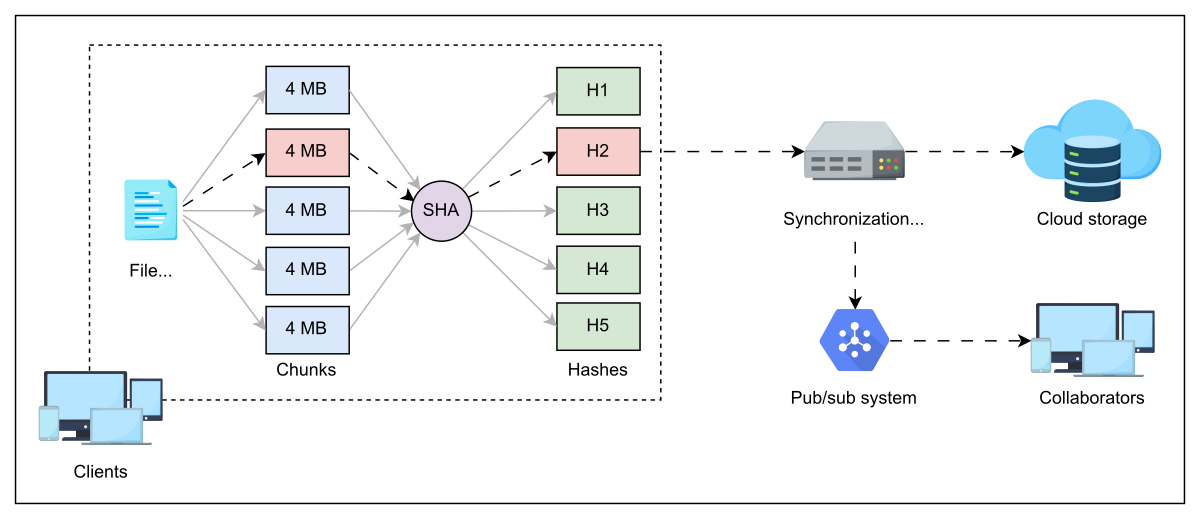
\includegraphics[width=0.5\textwidth]{Images/chapter_45/section_6405132675579904/4831707997798400.png}
 \caption{The modified chunk is uploaded to the cloud storage and sent to other clients via pub/sub system}
\end{figure}

When it comes to handling large files and network interruptions, the block-level sync algorithm provides resilience and efficiency.
\\
For large files, the client can upload or download chunks independently, meaning if there's a network interruption, the sync engine can resume from the last successfully uploaded or downloaded chunk rather than restarting the entire process.
\\
This chunked approach is critical for users on unreliable networks or with bandwidth constraints. Dropbox also uses~delta synchronization(Delta synchronization identifies and synchronizes the actual changes (deltas) between file versions, often at a finer level (e.g., byte or line-level). It 's more granular and flexible than block-level sync, which divides files into fixed-size blocks and syncs only modified blocks. Delta sync offers more precision, while block-level sync is simpler and more rigid.), ensuring that only modified chunks are synced, further optimizing the process.
\begin{quote}
\textbf{Note:} Dropbox uses an indexer to manage and search the stored files metadata, enabling quick retrieval and synchronization across devices.
\end{quote}

\begin{quote}
\textbf{Quiz:}
\textbf{Question 1:} When designing Dropbox's clients, which protocols or techniques should be used to efficiently monitor changes made by other clients?
\textbf{Answer:} Listening to changes made by other clients can be achieved through push notifications using long polling or WebSockets, allowing real-time updates without the need for constant polling. When a client modifies a file, the synchronization server detects the change and pushes notifications to all relevant clients. This keeps clients updated instantly with minimal network overhead. In cases of unreliable networks or idle periods, the system may employ periodic polling to ensure eventual consistency. This combination ensures efficient synchronization while balancing network resource usage.
\end{quote}

\subsubsection{Data storage and replication}\label{A0Kf1CjcJeTZz0myh7hQA}
\\
In Dropbox, data storage involves dividing files into smaller segments, or chunks, which are distributed across multiple storage servers for efficiency and scalability.
\\
Metadata is maintained separately to record the location and identifiers of these chunks, allowing for fast lookup and retrieval. Each chunk is encrypted before storage to ensure data confidentiality. To ensure durability and high availability, Dropbox replicates data chunks across multiple data centers.
\\
This replication provides redundancy and supports disaster recovery.
\\
If one data center becomes unavailable due to hardware failure or network issues, data can still be retrieved from another without interrupting service. While replication strengthens fault tolerance, it also introduces challenges. The system must provide low-latency access for users worldwide, manage eventual consistency across replicas, and address the operational complexity and costs associated with managing data across geographically distributed servers.

\subsubsection{Version control and conflict resolution}\label{XIvvBbOww0KehtaYFG8Pi}
\\
Dropbox allows multiple users to edit a document simultaneously, making version control and conflict resolution essential. The metadata server tracks file versions, storing previous copies for rollback if needed.
\\
A simple strategy is last-write-wins, where the most recent upload overwrites earlier changes. To prevent data loss, Dropbox can create conflicted copies for simultaneous edits, appending timestamps or usernames to distinguish versions. For text-based files, merge strategies can automatically combine non-conflicting changes, though complex conflicts may still require manual resolution.
\\
From a user perspective, the system notifies users of conflicts via the pub/sub system, allowing them to view and compare versions. The interface supports intuitive resolution, balancing automated handling with user control to manage conflicts efficiently without confusion.

\subsubsection{Security mechanisms}\label{W-l41zBBYBoNwjc3uL9uf}
\\
Dropbox implements robust security measures to protect user data both at rest and in transit.
\\
File chunks are encrypted using AES-256, while SSL/TLS ensures secure transmission, preventing interception or eavesdropping. The system also adheres to regulatory standards such as GDPR and HIPAA. GDPR compliance entails providing users with the ability to access, correct, and delete their data, as well as facilitating secure cross-border data transfers.
\\
HIPAA compliance requires encrypting protected health information (PHI) and supporting Business Associate Agreements (BAAs) with healthcare providers.

\subsection{Putting everything together}\label{XUqr7ywl4u1ypBixImK8q}
\\
The Dropbox system integrates multiple components and services to support efficient file storage, synchronization, and sharing.

\begin{figure}[htbp]
 \centering
 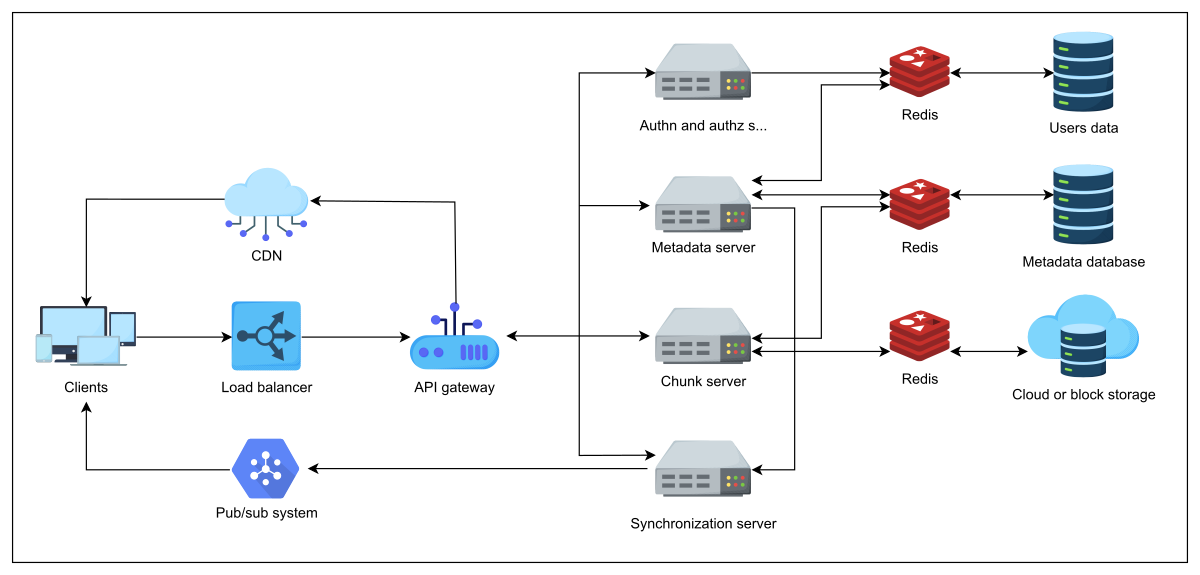
\includegraphics[width=0.5\textwidth]{Images/chapter_45/section_6405132675579904/4792424314306560.png}
 \caption{Detailed design of Dropbox system}
\end{figure}

\textbf{Components overview:}

\begin{itemize}
\item
\protect\phantomsection\label{DWReaR0APTK9nNf0EqY1J}
\textbf{Clients:} User devices with installed applications that interact with backend services to upload, download, and sync files.
\item
\protect\phantomsection\label{KnrSaz4ApjGtVQbZI-0BM}
\textbf{Load balancer:} Distributes incoming client traffic evenly across servers for efficient resource use.
\item
\protect\phantomsection\label{PWmsaLu8DjnWYVYc6Bigl}
\textbf{API gateway:} Entry point for client requests, routing them to the appropriate backend services.
\item
\protect\phantomsection\label{31FNRVTkMjfaU5LYkTrMX}
\textbf{CDN:} Delivers cached static content close to users to reduce latency.
\item
\protect\phantomsection\label{keyQHMObG1iA7NOJV-VDT}
\textbf{Authentication and authorization service (Authn/Authz):} Verifies user identity and enforces access control.
\item
\protect\phantomsection\label{QR6Rd9SXGk-vRa7rYUORC}
\textbf{File metadata server:} Maintains metadata (file names, paths, versions) and coordinates access to metadata databases and caches.
\item
\protect\phantomsection\label{EqjKxFxZDLOUDXplHze2o}
\textbf{Metadata database:} Stores file metadata, including locations and access permissions, typically in a NoSQL database.
\item
\protect\phantomsection\label{Waqt22gtKsdI7HOzswAtn}
\textbf{Chunk server:} Handles storage, retrieval, and management of file chunks efficiently.
\item
\protect\phantomsection\label{TikhLvSALn8Miosyrjfs2}
\textbf{Cloud or block storage:} Provides scalable storage for file chunks across distributed servers.
\item
\protect\phantomsection\label{eB-ffTbo6odhFteaY7wJ9}
\textbf{Synchronization server:} Tracks changes and ensures all clients have the latest file versions.
\item
\protect\phantomsection\label{H_iafs8jYguF7TkLpD3e7}
\textbf{Pub/sub system:} Publishes updates to subscribed clients, enabling real-time synchronization and notifications.
\end{itemize}
\begin{quote}
\textbf{Note:} User data and structured information, such as accounts or permissions, are stored in relational databases like MySQL.
\end{quote}
\subsection{Performance optimization}\label{ttXg01Np2fG84_i4AMEIS}
\\
Dropbox employs several techniques to improve system performance and ensure efficient file transfers.
\\
These methods include using redundant database servers, caching frequently accessed files, compressing file chunks during transfer, and applying data deduplication to avoid storing duplicate content. Network conditions---such as fluctuating bandwidth and latency---can significantly affect upload and download speeds.
\\
To mitigate these issues, Dropbox uses adaptive bandwidth control, multi-threaded transfers, and TCP optimizations that dynamically adjust transfer rates based on network quality.
\\
Storing local copies of frequently accessed files also helps reduce retrieval time and latency. Compression reduces the amount of data transmitted, while deduplication ensures that only unique file chunks are uploaded, resulting in faster and more efficient synchronization.
\\
Common compression algorithms include:

\begin{itemize}
\item
\protect\phantomsection\label{RwzpFYPnAXVF8zK40x20J}
Gzip (DEFLATE) for documents, JPEG for images, MP3 for audio
\item
\protect\phantomsection\label{gMKzcIEROsBVjUbA7d3ey}
LZ77 lossless compression
\item
\protect\phantomsection\label{aqLni5_j4v2IubxJI10d1}
On-the-fly algorithms such as LZMA, Snappy, and Brotli
\end{itemize}
\\
For deduplication, Dropbox can use:

\begin{itemize}
\item
\protect\phantomsection\label{yZOEKyFu_trm-TNdnZAz9}
SHA-256 hashing
\item
\protect\phantomsection\label{4HiZkrHioU0fMsKMJ8M3O}
MD5
\item
\protect\phantomsection\label{KueDPjxbVvOWsEVt8_z-w}
Rabin Fingerprinting
\item
\protect\phantomsection\label{eH2-SKEmLv7yYBRss_qWV}
Content-defined chunking (CDC)
\end{itemize}
\\
These strategies collectively enhance throughput, reduce storage costs, and improve user experience across devices.

\subsection{Conclusion}\label{fnoC6wElDKzhPVtx2B6Mq}
\\
The Dropbox design strikes a balance between functional efficiency and scalable architecture.
\\
File synchronization, version control, and access management are supported through chunking, hashing, and metadata management, ensuring reliability at scale. High availability, fault tolerance, and performance optimizations, including real-time updates and deduplication, provide consistent and efficient user experiences across devices.

% End of section content